\section* {2.1  Методы простой итерации и Ньютона}

\subsection{Постановка задачи}
Реализовать методы простой итерации и Ньютона решения нелинейных уравнений в виде программ, задавая в качестве входных данных точность вычислений. С использованием разработанного программного обеспечения найти положительный корень нелинейного уравнения (начальное приближение определить графически). Проанализировать зависимость погрешности вычислений от количества итераций.

{\bfseries Вариант:} 13

$ln(x+1)-2x+0.5=0$
%\pagebreak

\subsection{Результаты работы}
\begin{figure}[h!]
\centering
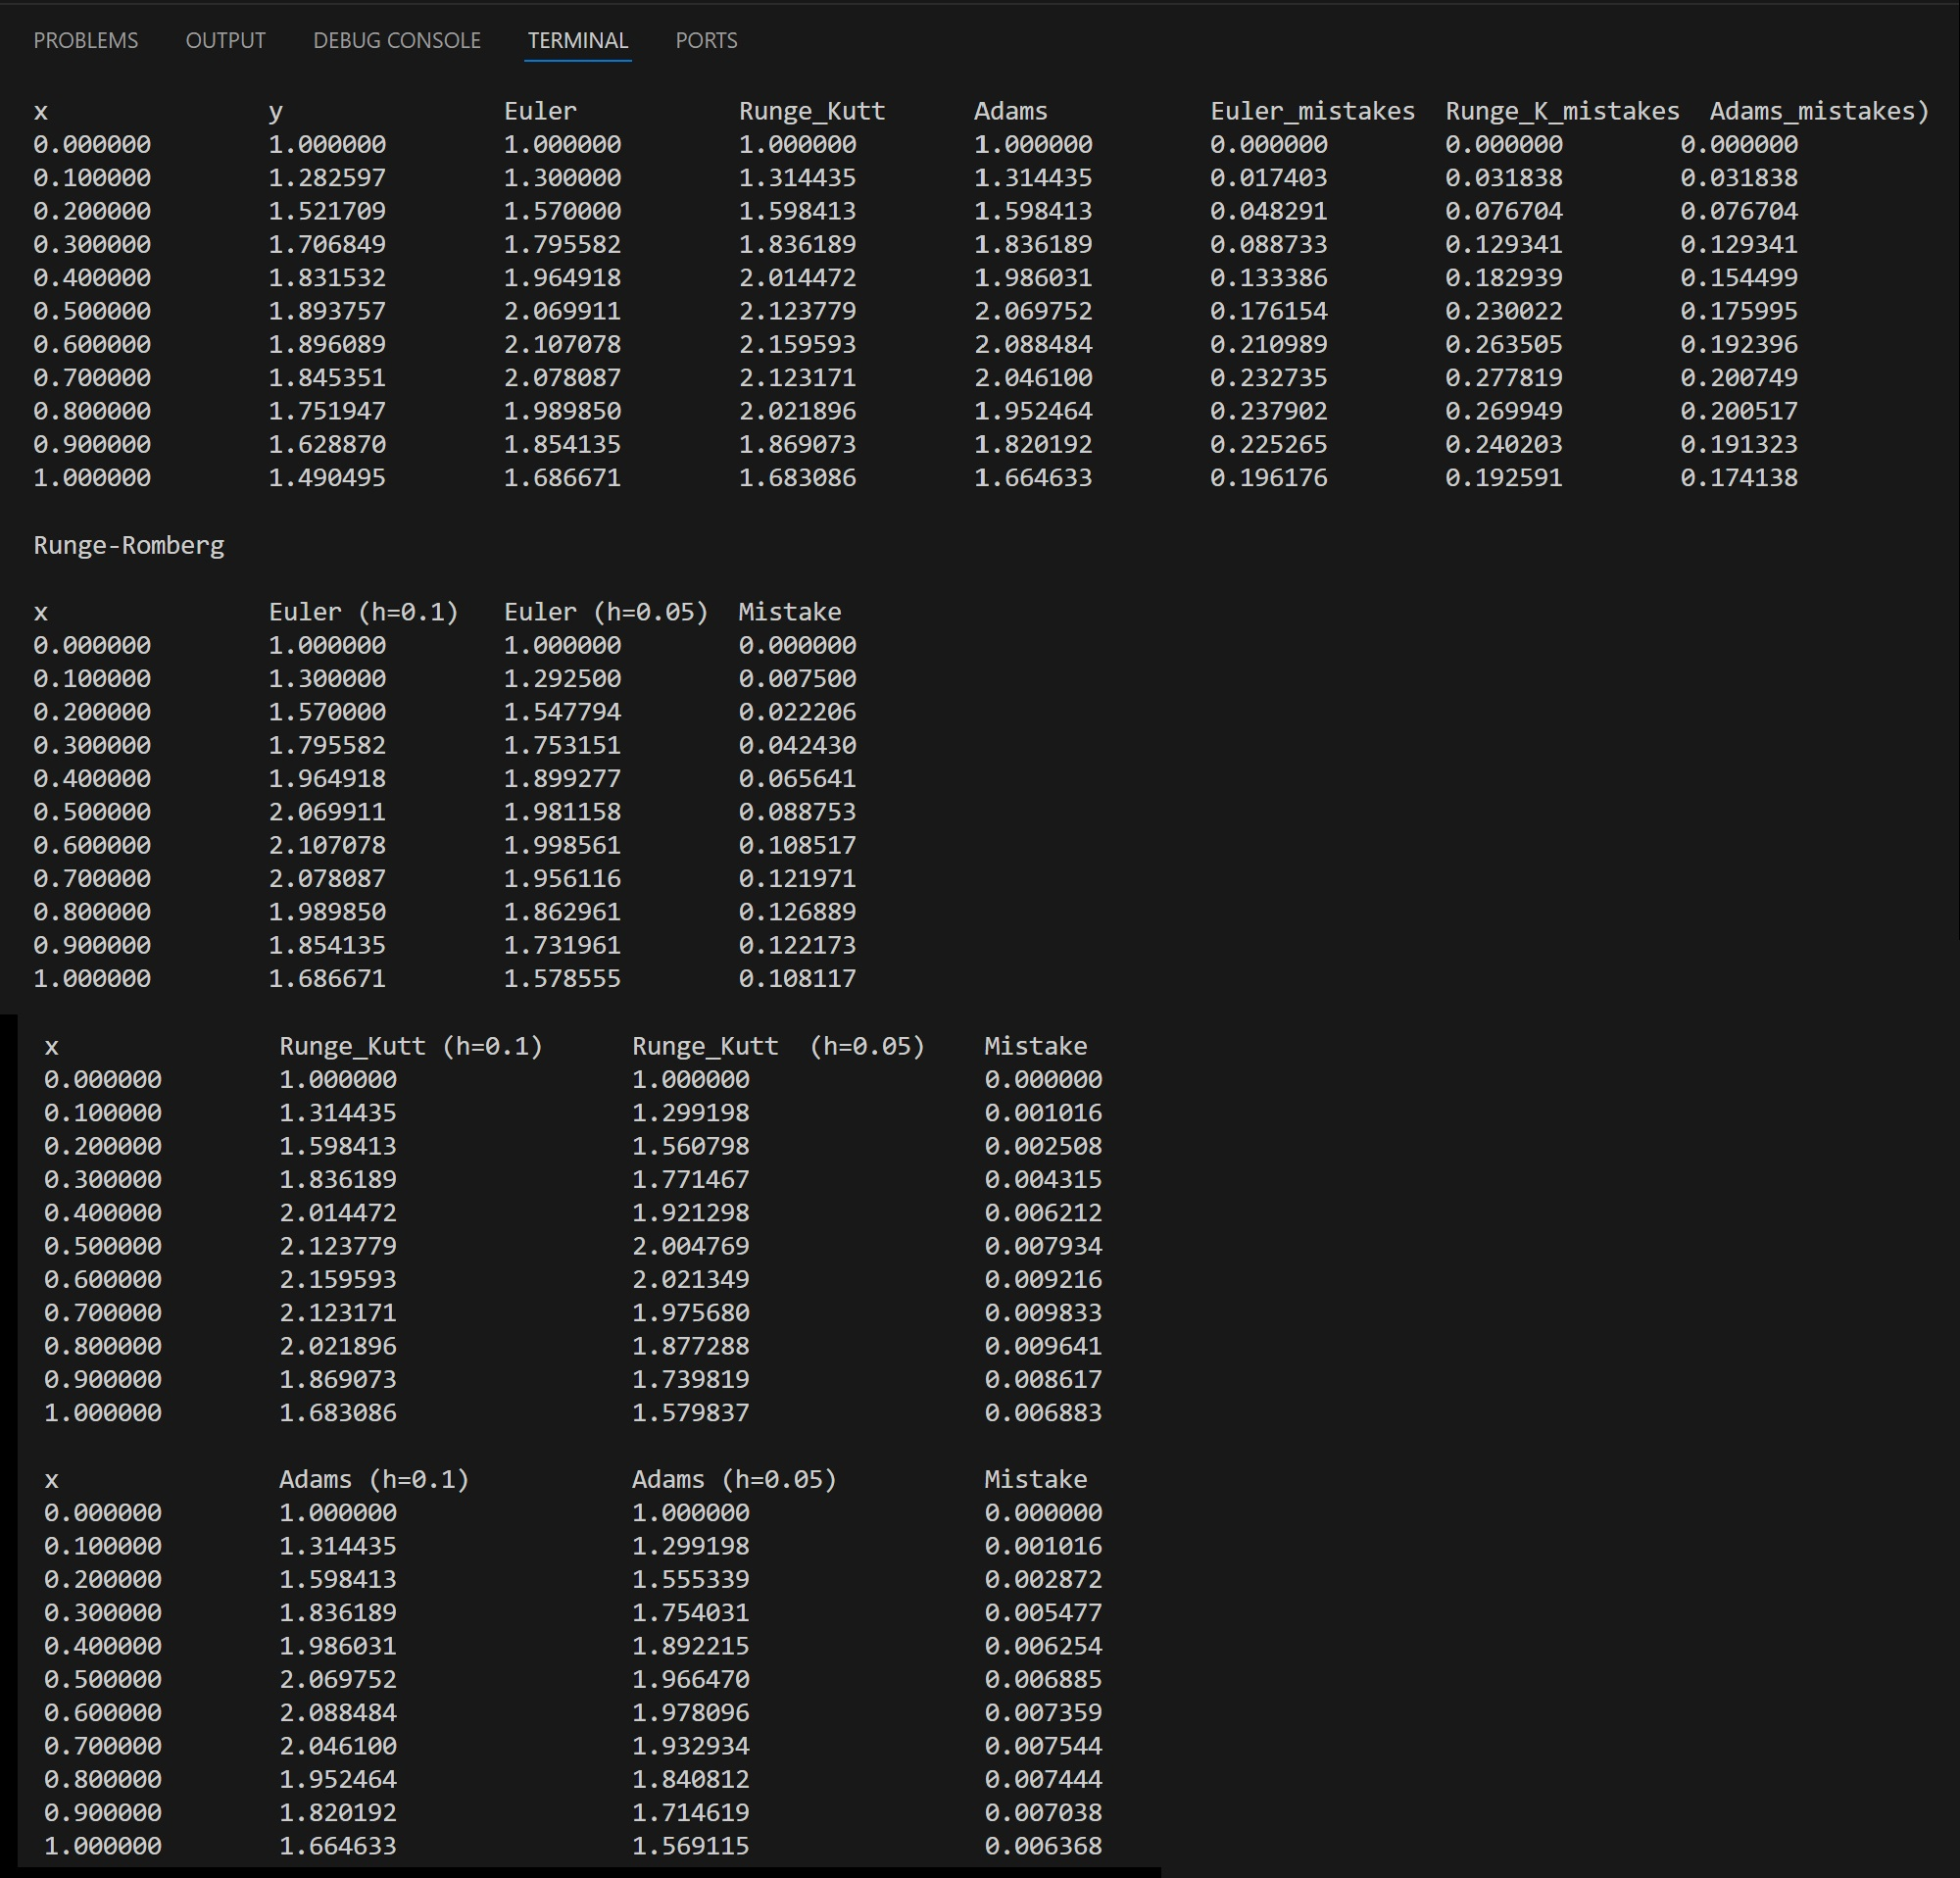
\includegraphics[width=12cm, height=6cm]{img_1}
\caption{Вывод программы в консоли}
\end{figure}
\pagebreak

\subsection{Исходный код}

\lstinputlisting{include/Lab_2.1.cpp}
\pagebreak

\section* {2.2  Методы простой итерации и Ньютона}

\subsection{Постановка задачи}
Реализовать методы простой итерации и Ньютона решения систем нелинейных уравнений в виде программного кода, задавая в качестве входных данных точность вычислений. С использованием разработанного программного обеспечения решить систему нелинейных уравнений (при наличии нескольких решений найти то из них, в котором значения неизвестных являются положительными); начальное приближение определить графически. Проанализировать зависимость погрешности вычислений от количества итераций. 

{\bfseries Вариант:} 13

\begin{cases}
& ((x_1)^2)/4+(x_2)^2 = 1 \\
& 2x_2-e^(x_1) = 0 \\
\end{cases}
%\pagebreak

\subsection{Результаты работы}
\begin{figure}[h!]
\centering
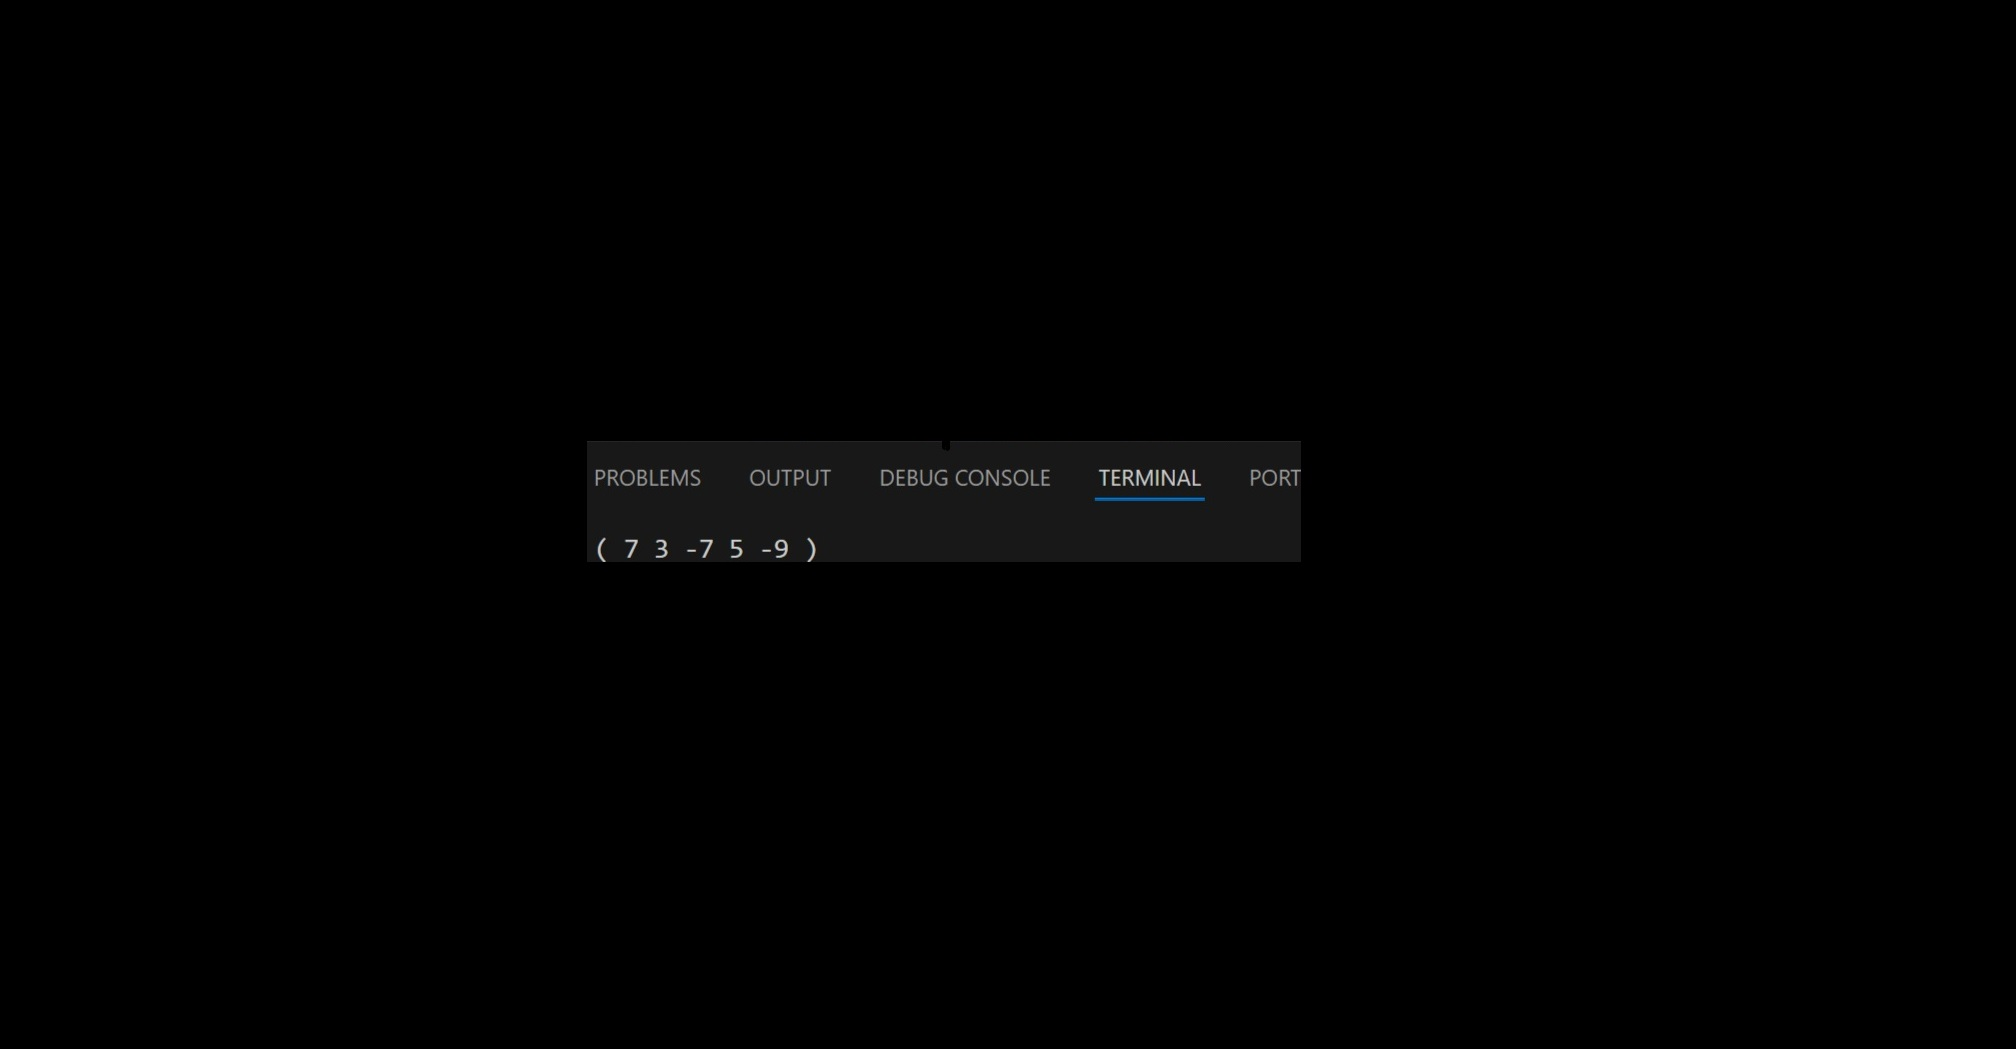
\includegraphics[width=15cm, height=6cm]{img_2}
\caption{Вывод программы в консоли}
\end{figure}
\pagebreak


\subsection{Исходный код}

\lstinputlisting{include/read.h}
\lstinputlisting{include/base.c}
\lstinputlisting{include/Lab_2.2.cpp}
